%! Compiler = pdflatex
%! BibTeX Compiler = biber
%TC:ignore - ignoriert die folgnden Wörter beim Wordcount in Overleaf
%-----------------------------------
% Define document and include general packages
%-----------------------------------
% Tabellen- und Abbildungsverzeichnis stehen normalerweise nicht im
% Inhaltsverzeichnis. Gleiches gilt für das Abkürzungsverzeichnis (siehe unten).
% Manche Dozenten bemängeln das. Die Optionen 'listof=totoc,bibliography=totoc'
% geben das Tabellen- und Abbildungsverzeichnis im Inhaltsverzeichnis (toc=Table
% of Content) aus.
% Da es aber verschiedene Regelungen je nach Dozent geben kann, werden hier
% beide Varianten dargestellt.
\documentclass[12pt,oneside,titlepage,listof=totoc,bibliography=totoc]{scrartcl}
%\documentclass[12pt,oneside,titlepage]{scrartcl}

%-----------------------------------
% Dokumentensprache
%-----------------------------------
\def\FOMEN{}% Auskommentieren um die Dokumentensprache auf englisch zu ändern
\newif\ifde
\newif\ifen

%-----------------------------------
% Meta informationen
%-----------------------------------
%-----------------------------------
% Meta Informationen zur Arbeit
%-----------------------------------

% Autor
\newcommand{\myAutor}{Dominik Fey}

% Adresse
\newcommand{\myAdresse}{Buschgasse 40 \\ \> \> \> 50189 Elsdorf}

% Titel der Arbeit
\newcommand{\myTitel}{Implementation of an AI-Supported Centralized Procurement Interface to Enhance Procurement
Processes in a Large-Scale Enterprise}

% Betreuer
\newcommand{\myBetreuer}{Prof. Dr. Bernd Ulmann}

% Lehrveranstaltung
\newcommand{\myLehrveranstaltung}{Bachelor Module}

% Matrikelnummer
\newcommand{\myMatrikelNr}{601373}

% Ort
\newcommand{\myOrt}{Cologne}

% Datum der Abgabe
\newcommand{\myAbgabeDatum}{\today}

% Semesterzahl
\newcommand{\mySemesterZahl}{7}

% Name der Hochschule
\newcommand{\myHochschulName}{FOM University of Applied Sciences for Economics and Management}

% Standort der Hochschule
\newcommand{\myHochschulStandort}{Cologne}

% Studiengang
\newcommand{\myStudiengang}{Business Informatics}

% Art der Arbeit
\newcommand{\myThesisArt}{Bachelor Thesis}

% Zu erlangender akademische Grad
\newcommand{\myAkademischerGrad}{Bachelor of Science (B.Sc.)}

% Firma
\newcommand{\myFirma}{Deutsche Telekom AG}

% Definition der Sprache
\ifdefined\FOMEN
%Englisch
\entrue
\usepackage[english]{babel}
\else
%Deutsch
\detrue
\usepackage[ngerman]{babel}
\fi


\newcommand{\langde}[1]{%
   \ifde\selectlanguage{ngerman}#1\fi}
\newcommand{\langen}[1]{%
   \ifen\selectlanguage{english}#1\fi}
\usepackage[utf8]{luainputenc}
\langde{\usepackage[babel,german=quotes]{csquotes}}
\langen{\usepackage[babel,english=british]{csquotes}}
\ifde\usepackage[ngerman]{babel}\fi
\usepackage[T1]{fontenc}
\usepackage{fancyhdr}
\usepackage{fancybox}
\usepackage[a4paper, left=4cm, right=2cm, top=4cm, bottom=2cm]{geometry}
\usepackage{graphicx}
\usepackage{colortbl}
\usepackage[capposition=top]{floatrow}
\usepackage{array}
\usepackage{float}      %Positionierung von Abb. und Tabellen mit [H] erzwingen
\usepackage{footnote}
% Darstellung der Beschriftung von Tabellen und Abbildungen (Leitfaden S. 44)
% singlelinecheck=false: macht die Caption linksbündig (statt zentriert)
% labelfont auf fett: (Tabelle x.y:, Abbildung: x.y)
% font auf fett: eigentliche Bezeichnung der Abbildung oder Tabelle
% Fettschrift laut Leitfaden 2018 S. 45
\usepackage[singlelinecheck=false, labelfont=bf, font=bf]{caption}
\usepackage{caption}
\usepackage{pdfpages}
\usepackage{enumitem}
\usepackage{amssymb}
\usepackage{mathptmx}
\usepackage{minted} %Kann für schöneres Syntax Highlighting genutzt werden. ACHTUNG: Python muss installiert sein.
\usepackage[scaled=0.9]{helvet} % Behebt, zusammen mit Package courier, pixelige Überschriften. Ist, zusammen mit mathptx, dem times-Package vorzuziehen. Details: https://latex-kurs.de/fragen/schriftarten/Times_New_Roman.html
\usepackage{courier}
\usepackage{amsmath}
\usepackage[table]{xcolor}
\usepackage{marvosym}			% Verwendung von Symbolen, z.B. perfektes Eurozeichen

\renewcommand\familydefault{\sfdefault}
\usepackage{ragged2e}

% Mehrere Fussnoten nacheinander mit Komma separiert
\usepackage[hang,multiple]{footmisc}
\setlength{\footnotemargin}{1em}

% to_do Aufgaben als Kommentare verfassen für verschiedene Editoren
\usepackage{todonotes}

% Verhindert, dass nur eine Zeile auf der nächsten Seite steht
\setlength{\marginparwidth}{2cm}
\usepackage[all]{nowidow}

%-----------------------------------
% Farbdefinitionen
%-----------------------------------
\definecolor{darkblack}{rgb}{0,0,0}
\definecolor{dunkelgrau}{rgb}{0.8,0.8,0.8}
\definecolor{hellgrau}{rgb}{0.0,0.7,0.99}
\definecolor{mauve}{rgb}{0.58,0,0.82}
\definecolor{dkgreen}{rgb}{0,0.6,0}

%-----------------------------------
% Pakete für Tabellen
%-----------------------------------
\usepackage{epstopdf}
\usepackage{nicefrac} % Brüche
\usepackage{multirow}
\usepackage{rotating} % vertikal schreiben
\usepackage{mdwlist}
\usepackage{tabularx}% für Breitenangabe

%-----------------------------------
% sauber formatierter Quelltext
%-----------------------------------
\usepackage{listings}
% JavaScript als Sprache definieren:
\lstdefinelanguage{JavaScript}{
	keywords={break, super, case, extends, switch, catch, finally, for, const, function, try, continue, if, typeof, debugger, var, default, in, void, delete, instanceof, while, do, new, with, else, return, yield, enum, let, await},
	keywordstyle=\color{blue}\bfseries,
	ndkeywords={class, export, boolean, throw, implements, import, this, interface, package, private, protected, public, static},
	ndkeywordstyle=\color{darkgray}\bfseries,
	identifierstyle=\color{black},
	sensitive=false,
	comment=[l]{//},
	morecomment=[s]{/*}{*/},
	commentstyle=\color{purple}\ttfamily,
	stringstyle=\color{red}\ttfamily,
	morestring=[b]',
	morestring=[b]"
}

\lstset{
	%language=JavaScript,
	numbers=left,
	numberstyle=\tiny,
	numbersep=5pt,
	breaklines=true,
	showstringspaces=false,
	frame=l ,
	xleftmargin=5pt,
	xrightmargin=5pt,
	basicstyle=\ttfamily\scriptsize,
	stepnumber=1,
	keywordstyle=\color{blue},          % keyword style
  	commentstyle=\color{dkgreen},       % comment style
  	stringstyle=\color{mauve}         % string literal style
}

%-----------------------------------
%Literaturverzeichnis Einstellungen
%-----------------------------------

% Biblatex

\usepackage{url}
\urlstyle{same}

%%%% Neuer Leitfaden (2018)
\usepackage[
backend=biber,
%style=ext-authoryear-ibid, % Auskommentieren und nächste Zeile einkommentieren, falls "Ebd." (ebenda) nicht für sich-wiederholende Fussnoten genutzt werden soll.
style=ext-authoryear,
maxcitenames=3,	% mindestens 3 Namen ausgeben bevor et. al. kommt
maxbibnames=999,
mergedate=false,
date=iso,
seconds=true, %werden nicht verwendet, so werden aber Warnungen unterdrückt.
urldate=iso,
innamebeforetitle,
dashed=false,
autocite=footnote,
doi=false,
useprefix=true, % 'von' im Namen beachten (beim Anzeigen)
mincrossrefs = 1
]{biblatex}%iso dateformat für YYYY-MM-DD

%weitere Anpassungen für BibLaTex
\input{skripte/modsBiblatex2018}

%%%%% Alter Leitfaden. Ggf. Einkommentieren und Bereich hierüber auskommentieren
%\usepackage[
%backend=biber,
%style=numeric,
%citestyle=authoryear,
%url=false,
%isbn=false,
%notetype=footonly,
%hyperref=false,
%sortlocale=de]{biblatex}

%weitere Anpassungen für BibLaTex
%\input{skripte/modsBiblatex}

%%%% Ende Alter Leitfaden

%Bib-Datei einbinden
\addbibresource{literatur/literatur.bib}

% Zeilenabstand im Literaturverzeichnis ist Einzeilig
% siehe Leitfaden S. 14
\AtBeginBibliography{\singlespacing}

%-----------------------------------
% Silbentrennung (Vgl. Leitfaden S.17) 
%-----------------------------------
\usepackage{hyphsubst}
\HyphSubstIfExists{ngerman-x-latest}{%
\HyphSubstLet{ngerman}{ngerman-x-latest}}{}
\usepackage{microtype}

\hyphenpenalty=5000 % Minimiert die Trennung
\exhyphenpenalty=5000 % Minimiert die Trennung am Zeilenende

%-----------------------------------
% Pfad fuer Abbildungen
%-----------------------------------
\graphicspath{{./}{./abbildungen/}}

%-----------------------------------
% Weitere Ebene einfügen
%-----------------------------------
\input{skripte/weitereEbene}

%-----------------------------------
% Paket für die Nutzung von Anhängen
%-----------------------------------
\usepackage{appendix}

%-----------------------------------
% Zeilenabstand 1,5-zeilig
%-----------------------------------
\usepackage{setspace}
\onehalfspacing

%-----------------------------------
% Absätze durch eine neue Zeile
%-----------------------------------
\setlength{\parindent}{0mm}
\setlength{\parskip}{0.8em plus 0.5em minus 0.3em}

\sloppy					%Abstände variieren
\pagestyle{headings}

%----------------------------------
% Präfix in das Abbildungs- und Tabellenverzeichnis aufnehmen, statt nur der Nummerierung (siehe Issue #206).
%----------------------------------
\KOMAoption{listof}{entryprefix} % Siehe KOMA-Script Doku v3.28 S.153
\BeforeStartingTOC[lof]{\renewcommand*\autodot{:}} % Für den Doppelpunkt hinter Präfix im Abbildungsverzeichnis
\BeforeStartingTOC[lot]{\renewcommand*\autodot{:}} % Für den Doppelpunkt hinter Präfix im Tabellenverzeichnis

%-----------------------------------
% Abkürzungsverzeichnis
%-----------------------------------
\usepackage[printonlyused]{acronym}

%-----------------------------------
% Symbolverzeichnis
%-----------------------------------
% Quelle: https://www.namsu.de/Extra/pakete/Listofsymbols.pdf
\usepackage[final]{listofsymbols}

%-----------------------------------
% Glossar
%-----------------------------------
\usepackage{glossaries}
\glstoctrue %Auskommentieren, damit das Glossar nicht im Inhaltsverzeichnis angezeigt wird.
\makenoidxglossaries
\newglossaryentry{NLU}{name={NLU},description={Das ist Natural Language Understanding.}}
\newglossaryentry{NLP}{name={NLP},description={Das ist Natural Language Processing.}}


%-----------------------------------
% PDF Meta Daten setzen
%-----------------------------------
\usepackage[hyperfootnotes=false]{hyperref} %hyperfootnotes=false deaktiviert die Verlinkung der Fußnote. Ansonsten inkompaibel zum Paket "footmisc"
% Behebt die falsche Darstellung der Lesezeichen in PDF-Dateien, welche eine Übersetzung besitzen
% siehe Issue 149
\makeatletter
\pdfstringdefDisableCommands{\let\selectlanguage\@gobble}
\makeatother

\hypersetup{
    pdfinfo={
        Title={\myTitel},
        Subject={\myStudiengang},
        Author={\myAutor},
        Build=1.1
    }
}

%-----------------------------------
% PlantUML
%-----------------------------------
%\usepackage{plantuml}

%-----------------------------------
% Umlaute in Code korrekt darstellen
% siehe auch: https://en.wikibooks.org/wiki/LaTeX/Source_Code_Listings
%-----------------------------------
\lstset{literate=
	{á}{{\'a}}1 {é}{{\'e}}1 {í}{{\'i}}1 {ó}{{\'o}}1 {ú}{{\'u}}1
	{Á}{{\'A}}1 {É}{{\'E}}1 {Í}{{\'I}}1 {Ó}{{\'O}}1 {Ú}{{\'U}}1
	{à}{{\`a}}1 {è}{{\`e}}1 {ì}{{\`i}}1 {ò}{{\`o}}1 {ù}{{\`u}}1
	{À}{{\`A}}1 {È}{{\'E}}1 {Ì}{{\`I}}1 {Ò}{{\`O}}1 {Ù}{{\`U}}1
	{ä}{{\"a}}1 {ë}{{\"e}}1 {ï}{{\"i}}1 {ö}{{\"o}}1 {ü}{{\"u}}1
	{Ä}{{\"A}}1 {Ë}{{\"E}}1 {Ï}{{\"I}}1 {Ö}{{\"O}}1 {Ü}{{\"U}}1
	{â}{{\^a}}1 {ê}{{\^e}}1 {î}{{\^i}}1 {ô}{{\^o}}1 {û}{{\^u}}1
	{Â}{{\^A}}1 {Ê}{{\^E}}1 {Î}{{\^I}}1 {Ô}{{\^O}}1 {Û}{{\^U}}1
	{œ}{{\oe}}1 {Œ}{{\OE}}1 {æ}{{\ae}}1 {Æ}{{\AE}}1 {ß}{{\ss}}1
	{ű}{{\H{u}}}1 {Ű}{{\H{U}}}1 {ő}{{\H{o}}}1 {Ő}{{\H{O}}}1
	{ç}{{\c c}}1 {Ç}{{\c C}}1 {ø}{{\o}}1 {å}{{\r a}}1 {Å}{{\r A}}1
	{€}{{\EUR}}1 {£}{{\pounds}}1 {„}{{\glqq{}}}1
}

%-----------------------------------
% Kopfbereich / Header definieren
%-----------------------------------
\pagestyle{fancy}
\fancyhf{}
% Seitenzahl oben, mittig, mit Strichen beidseits
% \fancyhead[C]{-\ \thepage\ -}

% Seitenzahl oben, mittig, entsprechend Leitfaden ohne Striche beidseits
\fancyhead[C]{\thepage}
%\fancyhead[L]{\leftmark}							% kein Footer vorhanden
% Waagerechte Linie unterhalb des Kopfbereiches anzeigen. Laut Leitfaden ist
% diese Linie nicht erforderlich. Ihre Breite kann daher auf 0pt gesetzt werden.
\renewcommand{\headrulewidth}{0.4pt}
%\renewcommand{\headrulewidth}{0pt}

%-----------------------------------
% Damit die hochgestellten Zahlen auch auf die Fußnote verlinkt sind (siehe Issue 169)
%-----------------------------------
\hypersetup{colorlinks=true, breaklinks=true, linkcolor=darkblack, citecolor=darkblack, menucolor=darkblack, urlcolor=darkblack, linktoc=all, bookmarksnumbered=false, pdfpagemode=UseOutlines, pdftoolbar=true}
\urlstyle{same}%gleiche Schriftart für den Link wie für den Text

%-----------------------------------
% Start the document here:
%-----------------------------------
\begin{document}

\pagenumbering{Roman}								% Seitennumerierung auf römisch umstellen
\newcolumntype{C}{>{\centering\arraybackslash}X}	% Neuer Tabellen-Spalten-Typ:
%Zentriert und umbrechbar

%-----------------------------------
% Textcommands
%-----------------------------------
\input{skripte/textcommands}

%-----------------------------------
% Titlepage
%-----------------------------------
\input{kapitel/titelseite}

%-----------------------------------
% Vorwort (optional; bei Verwendung beide Zeilen entkommentieren und unter Inhaltsverzeichnis setcounter entsprechend anpassen)
%-----------------------------------
%\input{kapitel/vorwort/vorwort}
%\newpage

%-----------------------------------
% Inhaltsverzeichnis
%-----------------------------------
% Um das Tabellen- und Abbbildungsverzeichnis zu de/aktivieren ganz oben in Documentclass schauen
\setcounter{page}{2}
\addtocontents{toc}{\protect\enlargethispage{-20mm}}% Die Zeile sorgt dafür, dass das Inhaltsverzeichnisseite auf die zweite Seite gestreckt wird und somit schick aussieht. Das sollte eigentlich automatisch funktionieren. Wer rausfindet wie, kann das gern ändern.
\setcounter{tocdepth}{4}
\tableofcontents
\newpage

%-----------------------------------
% Abbildungsverzeichnis
%-----------------------------------
\listoffigures
\newpage
%-----------------------------------
% Tabellenverzeichnis
%-----------------------------------
\listoftables
\newpage
%-----------------------------------
% Abkürzungsverzeichnis
%-----------------------------------
% Falls das Abkürzungsverzeichnis nicht im Inhaltsverzeichnis angezeigt werden soll
% dann folgende Zeile auskommentieren.
\addcontentsline{toc}{section}{\abbreHeadingName}

\section*{\langde{Abkürzungsverzeichnis}\langen{List of Abbreviations}}

\begin{acronym}[MVP]\itemsep0pt %der Parameter in Klammern sollte die längste Abkürzung sein. Damit wird der Abstand zwischen Abkürzung und Übersetzung festgelegt
  \acro{API}{Application Programming Interface}
  \acro{IaC}{Infrastructure-as-Code}
  \acro{MVP}{Minimum Viable Product}
  \acro{NLP}{Natural Language Processing}
  \acro{NLU}{Natural Language Understanding}
\end{acronym}
\newpage

%-----------------------------------
% Symbolverzeichnis
%-----------------------------------
% In Overleaf führt der Einsatz des Symbolverzeichnisses zu einem Fehler, der aber ignoriert werdne kann
% Falls das Symbolverzeichnis nicht im Inhaltsverzeichnis angezeigt werden soll
% dann folgende Zeile auskommentieren.
\phantomsection\addcontentsline{toc}{section}{\symheadingname}
\input{skripte/symbolDef}
\listofsymbols
\newpage

%-----------------------------------
% Glossar
%-----------------------------------
\printnoidxglossaries
\newpage

%-----------------------------------
% Sperrvermerk
%-----------------------------------
\input{kapitel/anhang/sperrvermerk}

%-----------------------------------
% Seitennummerierung auf arabisch und ab 1 beginnend umstellen
%-----------------------------------
\pagenumbering{arabic}
\setcounter{page}{1}

%-----------------------------------
% Kapitel / Inhalte
%-----------------------------------
%TC:endignore - berücksichtigt die folgnden Wörter beim Wordcount in Overleaf
% Die Kapitel werden über folgende Datei eingebunden
% Hinzugefügt aufgrund von Issue 167
%-----------------------------------
% Kapitel / Inhalte
%-----------------------------------
\section{Relevance}\label{sec:Relevance}
Dies soll eine \LaTeX{}-Vorlage für den persönlichen Gebrauch werden. Sie hat weder einen Anspruch auf Richtigkeit, noch
auf Vollständigkeit. Die Quellen liegen auf Github zur allgemeinen Verwendung. Verbesserungen sind jederzeit willkommen.

\subsection{Objective}\label{subsec:objective}
Kleiner Reminder für mich in Bezug auf die Dinge, die wir bei der Thesis beachten sollten und \LaTeX{}
-Vorlage für die Thesis.

\subsection{Structure of the Paper}\label{subsec:structure-of-the-paper}
Kapitel~\ref{sec:fundamentals}
enthält die Inhalte des Thesis-Days und alles, was zum inhaltlichen erstellen der Thesis relevant sein könnte.
In
Kapitel~\ref{sec:methodology}~\nameref{sec:methodology} findet ihr wichtige Anmerkungen zu \LaTeX{}
, wobei die wirklich wichtigen Dinge im Quelltext dieses Dokumentes stehen (siehe auch die Verzeichnisstruktur in
Abbildung.

\subsection{Technical Stack Relevance}\label{subsec:technical-stack-relevance}

The selection of a robust and integrated technical stack is pivotal for the successful implementation of sophisticated
software solutions, particularly when developing a chatbot designed to understand and fulfill complex customer needs.
The project presented in this bachelor’s thesis involves the creation of a chatbot that leverages \ac{NLP} to interpret
customer inquiries and match them with relevant items from a supplier catalog. To achieve this, the backend relies on
Python and Haystack, while the frontend utilizes Vue, and the deployment is managed through containerization and
orchestration technologies like Docker and Kubernetes.

\subsubsection{Backend Technologies}

Python serves as the backbone of the application due to its extensive ecosystem and its ability to seamlessly integrate
various libraries and frameworks that facilitate rapid prototyping and the development of complex data-driven
functionalities.\autocite[cf.][p. 12]{shrivastavaDesignImplementationChatbot}
\autocite[cf.][pp. 240--241]{christensenPythonPipelineRapid2022} Its prominence in the fields of machine
learning and data science makes it an ideal choice for implementing a chatbot that requires advanced \ac{NLU}
capabilities.\autocite[cf.][p. 1]{lortiePythonModernData2022}\autocite[cf.][p. 85]{joshiOverviewPythonLibraries}
Specifically, Python's compatibility with \acs{NLP} frameworks like Haystack and many libraries ensures that
the chatbot can parse user inputs and perform context-aware semantic searches.
\autocite[cf.][p. 21]{fareezPOPULARPYTHONLIBRARIES2020} This capability is crucial for accurately interpreting customer
needs and mapping them to appropriate products or services in the supplier catalog.

The integration of Haystack within this project serves as a cornerstone for the development of an intelligent,
search-driven chatbot, which is designed to address the intricate nature of customer inquiries. Haystack, a robust
open-source \acs{NLP} framework, employs a sophisticated Reader-Retriever architecture that
harmonizes the capabilities of both information retrieval and deep semantic understanding. This dual approach
capitalizes on advanced \acs{NLP} methodologies to enhance the chatbot’s performance in extracting pertinent information
from extensive datasets\autocite[cf.][p. 236]{krishnamoorthyEvolutionReadingComprehension2021}.

Notably, rather than utilizing the standard BERT model, this implementation leverages OpenAI’s GPT-4o model within the
Haystack framework. This allows the system to engage in nuanced contextual interpretation, thereby significantly
improving the precision of semantic searches. The choice of GPT-4o is particularly advantageous in question-answering
scenarios, as it allows the chatbot to comprehend the subtleties of customer queries and generate responses that are not
only contextually relevant but also demonstrate a high degree of language understanding
\autocite[cf.][pp. 943--944]{syedQuestionAnsweringChatbot2021}.

Moreover, Haystack’s modular architecture and extensible \acp{API} offer a high degree of flexibility, facilitating
seamless integration within the chatbot’s overall architecture. This ensures that the processes of searching and
retrieving supplier catalog data are executed with optimal accuracy and efficiency. Consequently, Haystack’s inclusion
in the technical stack is not merely contributory to the current system’s capabilities but also establishes a solid
foundation for prospective advancements and refinements in the chatbot’s functional repertoire.


The backend system also incorporates PostgreSQL as its database solution. PostgreSQL’s support for complex queries and
its capability to handle structured data are essential for managing and accessing the supplier information and product
details stored within the system.\autocite[cf.][pp. 23--24]{abbasiAdaptiveScalableDatabase2024}
The integration of PostgreSQL ensures that the chatbot can quickly and efficiently
retrieve the necessary data, thereby reducing latency and enhancing the overall user experience.

For monitoring and observability, the project employs Langfuse and OpenTelemetry, which provide comprehensive tracing
and metrics collection across the microservices architecture.\autocite[cf.][p. 15014]{thakurReviewOpentelemetryHTTP2022}
This is particularly relevant given the experimental
nature of the prototype, where understanding system performance and identifying potential bottlenecks are crucial for
iterative development and refinement. By utilizing these tools, the project gains valuable insights into the behavior of
the chatbot, allowing for continuous improvement and optimization.

FastAPI serves as the web framework for the backend, offering a high-performance environment that supports asynchronous
programming.\autocite[cf.][p. 9]{chenModelAlgorithmResearch2023}
This choice is particularly relevant for the chatbot, as it enables handling multiple concurrent requests
with minimal overhead, ensuring that the application remains responsive even under heavy loads.

The project also leverages the \texttt{uv} package for dependency management and deployment configuration. \texttt{uv}
simplifies the process of configuring Python dependencies and allows for a smoother deployment process by ensuring
compatibility and consistency between various package versions.
\autocite[cf.][URL last accessed on 2024-10-05]{canorodriguezPythonPackagingGreat2024}

\subsubsection{Frontend Technologie}

On the frontend, Vue.js and Vuetify are utilized to create an intuitive and responsive user interface.
The decision to use Vue.js stems from its reactive nature and modular architecture, which align with the need for a
maintainable and easily extensible codebase.\autocite[cf.][p. 268]{kaluzaComparisonFrontendFrameworks2018}
\autocite[cf.][pp. 1--2]{liResearchSinglePage2021} It is effective for developing a chatbot interface that needs to
present complex data in an accessible manner, while also allowing for dynamic updates based on user interactions.
\autocite[cf.][p. 493]{mokogintaDevelopingModernJavaScript2024}

\subsubsection{Deployment and Infrastructure Management}

Deployment is managed through a combination of Docker, Kubernetes, and Terraform.
Docker’s role in containerizing the application ensures that the entire software stack can be encapsulated and deployed
consistently across various environments.\autocite[cf.][p. 191]{openjaStudyingPracticesDeploying2022} This is essential
for a project like this, where different iterations of the prototype may need to be tested in different setups.
Kubernetes, in turn, provides the orchestration needed to manage these containers, allowing for automated scaling and
high availability.\autocite[cf.][pp. 2,7-8]{carrionKubernetesSchedulingTaxonomy2022} The use of Terraform as an \ac{IaC}
tool ensures that cloud resources can be provisioned and managed efficiently, providing a stable and reproducible
deployment environment.\autocite[cf.][p. 24]{n.EvaluatingDevopsTools2023}

\vspace{0,75cm}

In summary, each component of the technical stack has been carefully selected to meet the unique requirements of the
chatbot project.\ The combination of Python and Haystack provides robust \acs{NLP} capabilities for understanding and
processing user inputs, while FastAPI support real-time interactions. PostgreSQL ensures efficient data management,
and Langfuse and OpenTelemetry offer the necessary monitoring tools. On the frontend, Vue.js and Vuetify deliver a
responsive and interactive user interface, and the deployment stack, comprised of Docker, Kubernetes, and Terraform,
guarantees scalability and reliability. This cohesive selection of technologies forms a solid foundation for the
development of a chatbot that not only meets the functional requirements but also adheres to best practices in software
engineering.

\newpage
\section{Fundamentals}\label{sec:fundamentals}
\newpage


\section{Methodology}\label{sec:methodology}

\subsection{Requirements Engineering}\label{subsec:requirements-engineering}

\subsubsection{Introduction to Requirements Engineering According to Sommerville}

\ac{RE}, as outlined by Ian Sommerville, is a multifaceted process aimed at systematically defining a
system’s specifications. \autocite[cf.][p.5]{sommervilleRequirementsEngineeringGood1997} It comprises five
interconnected activities: Requirements Documentation, Requirements Elicitation, Requirements Analysis and Negotiation,
Requirements Validation, and Requirements Management.\autocite[cf.][p.11]{sommervilleRequirementsEngineeringGood1997}
Each activity has distinct objectives but collectively ensures the system satisfies both functional and non-functional
requirements.\autocite[cf.][p.7--8]{sommervilleRequirementsEngineeringGood1997}

Requirements Documentation serves as the foundation, formalizing needs, expectations, and constraints into a structured
format, such as a Software Requirements Specification. This document bridges communication between stakeholders
and developers and evolves with the project, supporting traceability and consistency. It is not merely a list of
requirements but provides contextual rationale for each, enhancing clarity and stakeholder alignment.
\autocite[cf.][38--40]{sommervilleRequirementsEngineeringGood1997}

The process begins with Requirements Elicitation, which involves proactively engaging with stakeholders, including
end-users and domain experts, to extract comprehensive requirements. Sommerville highlights this phase as an active
process of understanding the problem domain and reconciling conflicting needs through techniques like interviews,
workshops, and prototyping. This activity is vital for capturing all relevant requirements and establishing a shared
understanding of the system’s objectives.\autocite[cf.][p.64--65]{sommervilleRequirementsEngineeringGood1997}

Next, Requirements Analysis and Negotiation transforms these inputs into a coherent and conflict-free set of
requirements. Techniques such as modeling and prioritization help refine requirements, while negotiation resolves
trade-offs between competing stakeholder priorities. This ensures a balanced and agreed-upon set of requirements,
addressing concerns like performance versus cost or user flexibility versus security.
\autocite[cf.][p.112--113]{sommervilleRequirementsEngineeringGood1997}

Requirements Validation, a critical phase, ensures requirements reflect stakeholder needs and are feasible within
constraints. Using techniques such as formal inspections, peer reviews, and prototyping, validation identifies
ambiguities and contradictions early, minimizing costly changes later and ensuring the system aligns with stakeholder
expectations.\autocite[cf.][p.190--191]{sommervilleRequirementsEngineeringGood1997}

Requirements Management, the final activity, involves tracking and controlling changes as the project evolves.
Requirements are inherently dynamic, shifting with stakeholder understanding, new regulations, or market conditions.
Sommerville’s approach emphasizes maintaining traceability and documenting changes to ensure all modifications are
transparent and approved, reducing risks and maintaining requirement integrity.
\autocite[cf.][p.216--217]{sommervilleRequirementsEngineeringGood1997}

\subsubsection{Selection of Requirements Engineering Approach}

The selection of the \acs{RE} approach by Sommerville for this project was based on
tailoring each \acs{RE} activity to systematically uncover and refine requirements, thus providing a robust
methodological foundation.

For Requirements Documentation, Sommerville’s recommendations to "Define a Standard Document Structure" and "Make the
Document Easy to Change" were implemented. The standardized structure ensured clarity and traceability, while the
flexibility to modify the document supported iterative updates.
\autocite[cf.][p.41]{sommervilleRequirementsEngineeringGood1997}
\autocite[cf.][p.60]{sommervilleRequirementsEngineeringGood1997} This approach facilitated rigorous traceability, deemed
more critical for a prototype-focused project than alternatives like summarizing requirements, which prioritize
readability over the detailed documentation needed to manage evolving requirements.
\autocite[cf.][p.47]{sommervilleRequirementsEngineeringGood1997}

In Requirements Elicitation, the strategies "Use Scenarios to Elicit Requirements," "Define Operational Processes," and
"Prototyping Poorly Understood Requirements" were selected due to their effectiveness in refining complex and abstract
requirements through iterative development and visualization. "Use Scenarios to Elicit Requirements" enabled precise
visualization of user interactions, crucial for capturing the chatbot’s nuanced behavior.
\autocite[cf.][p.99]{sommervilleRequirementsEngineeringGood1997} "Define Operational Processes" provided a structured
method for visualizing workflows, ensuring accurate capture of procedural requirements, while "Prototype Poorly U
nderstood Requirements" translated ambiguous requirements into tangible artifacts for stakeholder discussions.
\autocite[cf.][p.102--103]{sommervilleRequirementsEngineeringGood1997}
\autocite[cf.][p.94--96]{sommervilleRequirementsEngineeringGood1997} These strategies were preferred over approaches
like "Collect Requirements From Multiple Viewpoints," as the prototype’s limited scope did not necessitate broad
stakeholder involvement from the outset.\autocite[cf.][p.90]{sommervilleRequirementsEngineeringGood1997}

For Requirements Analysis and Negotiation, the project adopted "Plan for Conflicts and Conflict Resolution" due to its
structured approach to identifying and resolving conflicting requirements.
\autocite[cf.][p.125--127]{sommervilleRequirementsEngineeringGood1997} This systematic method facilitated
discussions on competing priorities and consensus-building, making it more suitable than less structured alternatives
like "Define System Boundaries" or "Provide Software to Support Negotiations," which do not support the iterative,
dialogic nature of ongoing negotiations in prototype development.
\autocite[cf.][p.114]{sommervilleRequirementsEngineeringGood1997}
\autocite[cf.][p.121]{sommervilleRequirementsEngineeringGood1997}

The Requirements Validation phase applied "Organize Formal Requirements Inspections" and "Use Prototyping to Verify
Requirements." The former enabled comprehensive identification of inconsistencies through structured reviews, while the
latter facilitated visual validation and iterative feedback.
\autocite[cf.][p.195--196]{sommervilleRequirementsEngineeringGood1997}
\autocite[cf.][p.203--204]{sommervilleRequirementsEngineeringGood1997} The decision to forego "Define Validation
Checklists" was based on its less adaptable structure, which is not as effective for validating the evolving visual and
interactive components of the project.\autocite[cf.][p.200]{sommervilleRequirementsEngineeringGood1997}

Finally, in Requirements Management, "Define Policies for Requirements Management" was implemented to maintain
traceability and manage changes systematically. Establishing clear policies ensured that all requirements could be
efficiently tracked and modified in response to evolving project needs.
\autocite[cf.][p.221--222]{sommervilleRequirementsEngineeringGood1997} The project opted not to use a database for
managing requirements, focusing instead on robust change management policies to ensure a controlled and flexible
environment for reviewing and integrating changes. \autocite[cf.][p.236]{sommervilleRequirementsEngineeringGood1997}
This emphasis on policies over tools supported the dynamic nature of the prototype’s development while preserving
project coherence and stakeholder alignment.

\subsubsection{Application of Requirements Engineering in the Project}

The application of \acs{RE} in this project adhered to an iterative and collaborative methodology,
incorporating structured documentation, continuous stakeholder engagement, and interactive design tools to refine and
validate requirements throughout the development lifecycle. This approach, guided by Sommerville’s principles, enabled
effective communication, alignment, and feedback across all parties.

The foundation, the Requirements Documentation, began with a structured Word document containing a requirements table,
which served as the central repository for capturing, organizing, and updating requirements. This document ensured
systematic traceability and provided a consistent foundation for ongoing modifications as new insights emerged. The
example from \ac{IEEE}, mentioned in Sommerville's book, is not used, because for a Prototype it is to much.
\autocite[cf.][p.42--43]{sommervilleRequirementsEngineeringGood1997} A simpler version was created.

During Requirements Elicitation, workshops with domain experts were conducted to deepen understanding of the procurement
process and to capture core requirements. These sessions were complemented by ad-hoc meetings throughout development to
address emerging needs and clarify ambiguities. The elicitation phase leveraged iterative prototyping, progressing from
initial mockups in Miro to refined designs in Figma, and ultimately to functional screens in Vue. This incremental
approach allowed stakeholders to engage with evolving system representations, offering targeted feedback and further
refining requirements at each stage.

The Requirements Analysis and Negotiation phase synthesized feedback gathered during workshops and prototyping sessions.
Weekly meetings provided a forum to discuss and resolve conflicting priorities among stakeholders, while bi-weekly
management meetings ensured strategic alignment and secured high-level approval for changes. This continuous engagement
facilitated a dynamic negotiation process, allowing for re-prioritization and refinement of requirements based on
stakeholder feedback and evolving project constraints.

For Requirements Validation, a combination of systematic reviews and interactive prototyping was used. The prototypes,
evolving from initial sketches in Miro to detailed designs in Figma and implemented screens in Vue, enabled stakeholders
to visualize how their requirements would be realized, aiding in early identification of inconsistencies or
misalignments. Regular reviews ensured alignment between the documented requirements and the evolving system, minimizing
the risk of discrepancies.

Throughout Requirements Management, change control policies were strictly followed, ensuring that all requirement
modifications were systematically documented, reviewed, and approved. The structured requirements table was continuously
updated to reflect these changes, maintaining traceability and transparency. This disciplined approach to requirements
management preserved control over evolving requirements and ensured that stakeholders remained informed of any
adjustments.


\subsection{Prototyping}\label{subsec:prototyping}

\subsubsection{Introduction to the Prototyping Methodology According to Floyd}\label{subsubsec:ptintro}

The prototyping approach developed by Christiane Floyd represents a structured methodology used primarily in software
development to improve communication between developers and users, reduce misunderstandings, and ultimately enhance the
quality of the final product.\autocite[cf.][p.2--3]{floydSystematicLookPrototyping1984} This methodology provides an
alternative to the traditional linear, phase-oriented development process by introducing a dynamic element of iteration
and feedback.\autocite[cf.][p.3]{floydSystematicLookPrototyping1984} As a result, it facilitates a more
interactive and user-centered development process.\autocite[cf.][p.3--4]{floydSystematicLookPrototyping1984}

Floyd’s prototyping process is structured as a cyclical sequence of four distinct steps: functional selection,
construction, evaluation, and further use.\\ The first step, Functional Selection, involves identifying the specific
functions that the prototype should demonstrate. The selected functionalities are derived from the relevant work tasks
to ensure meaningful demonstrations, while acknowledging that the prototype does not need to represent the final product
comprehensively. This allows for a degree of flexibility in the selection and prioritization of features to be included
in the prototype.\autocite[cf.][p.4]{floydSystematicLookPrototyping1984}

The second step, Construction, entails building the prototype using techniques and tools that enable rapid development
and easy adjustments. At this stage, the focus is not on developing a fully functional system, but rather on
demonstrating and assessing specific aspects of the final product. This approach enables the prototype to act as a tool
for exploring different solutions and gathering feedback.\autocite[cf.][p.4]{floydSystematicLookPrototyping1984}

Evaluation, the third step in the process, serves as the cornerstone of the prototyping methodology. In this step,
feedback from all relevant stakeholders—including potential users—is collected and analyzed to refine and guide
subsequent development stages. This iterative process ensures that the prototype evolves in alignment with user
expectations and needs.\autocite[cf.][p.4--5]{floydSystematicLookPrototyping1984}

The final step, Further Use, determines the prototype's role after the evaluation phase. Depending on its effectiveness
and the degree to which it meets requirements, the prototype can be discarded, modified for continued use, or serve as a
foundation for the final product. This flexibility is critical in accommodating evolving requirements and objectives,
making the prototyping approach particularly valuable in contexts where specifications are expected to change
frequently.\autocite[cf.][p.5]{floydSystematicLookPrototyping1984}

Floyd’s methodology also categorizes prototyping into three primary approaches, each based on the goals and context of
development: exploratory prototyping, experimental prototyping, and evolutionary prototyping.
\autocite[cf.][p.6]{floydSystematicLookPrototyping1984}\\ Exploratory Prototyping is
primarily used to clarify requirements and foster creative cooperation between developers and users during the early
stages of development. It is particularly useful when there is a lack of clarity on the system’s final objectives, as it
allows for broad experimentation and refinement of ideas before committing to a specific solution.
\autocite[cf.][p.6--7]{floydSystematicLookPrototyping1984}

In contrast, Experimental Prototyping focuses on testing proposed solutions to validate specific hypotheses, such as
user interface design, system performance, or algorithm feasibility. This approach might involve techniques such as full
functional simulation or human interface simulation to verify that the proposed design meets the intended objectives.
\autocite[cf.][p.8--10]{floydSystematicLookPrototyping1984}

Finally, Evolutionary Prototyping treats the prototype as a system that continuously evolves to adapt to changing
requirements over time. Each version of the prototype serves as a basis for the next iteration, incorporating new
insights and user feedback. This approach is especially beneficial in scenarios where requirements are expected to
change frequently, rendering a static set of requirements impractical.
\autocite[cf.][p.10--12]{floydSystematicLookPrototyping1984}

To support these prototyping processes, various techniques and tools can be utilized.
\autocite[cf.][p.12]{floydSystematicLookPrototyping1984} \\Modular Design, for instance, encourages the use of small,
independent modules that can be replaced or refined as needed, thereby facilitating iterative development and easing
integration into the final product.\autocite[cf.][p.12]{floydSystematicLookPrototyping1984} \\Additionally, Dialogue
Design plays a crucial role in ensuring that the user interface is adaptable and transparent, which enables effective
evaluation and modification of the user experience.\autocite[cf.][p.12]{floydSystematicLookPrototyping1984}
\\Furthermore, Simulation techniques allow for simulating aspects of the final system that are not yet fully
implemented, enabling the assessment of system performance and user interaction without the need for a complete
implementation.\autocite[cf.][p.13]{floydSystematicLookPrototyping1984}

\subsubsection{Selection of Prototyping Approach}\label{subsubsec:ptselection}

Given the context and objectives of this project, the decision was made to adopt the experimental prototyping approach.
This choice is rooted in the fact that the project requirements have already been well-defined through a comprehensive
requirements engineering process, thus eliminating the need for exploratory prototyping. The clear specification of
functionalities and user expectations ensures that the focus can shift from understanding requirements to validating and
testing specific design choices.

Furthermore, the experimental approach is particularly well-suited for scenarios where a prototype is intended to serve
as a preliminary proof of concept rather than a foundation for incremental development. This aligns perfectly with the
anticipated lifecycle of the prototype in this project, which is expected to be discarded once the \ac{MVP} phase
begins. As the project moves towards the MVP stage, a fresh start will be made, incorporating only validated concepts
and findings from the experimental prototype. Therefore, evolutionary prototyping is not applicable, as it is primarily
designed for projects that involve iterative refinement and continuous evolution of the same prototype.

The experimental prototyping approach allows for focused experimentation with various design elements, interface
interactions, and technical implementations, all within a controlled environment that does not necessitate long-term
integration into the final product.

\subsubsection{Application of Experimental Prototyping in the Project}\label{subsubsec:ptapplication}

The experimental prototyping approach will be implemented in this project with a focus on validating user interface
designs, interactions, and core functionalities against predefined requirements. The development of the prototype will
leverage a set of carefully selected techniques that facilitate rapid iteration and feedback.

A key technique employed is simulation, which is used to mimic certain system behaviors without integrating the
prototype into live production environments. This decision is motivated by the limited scope of the prototype and the
intention to avoid disruptions to existing systems. By relying on test data instead of actual production data, the
prototype can simulate real-world scenarios and provide valuable insights into its performance and user experience.

Moreover, the prototype will not attempt to implement every function in its final depth and breadth. Instead, certain
features will be simulated to convey the look and feel of the system, providing a realistic representation of how the
final product would function. This is where Modular Design plays a crucial role. By leveraging modular design principles
, the prototype can separate the user interface from the underlying logic and backend functionalities. This allows
specific modules to be developed exclusively for the UI, simulating the presence of certain features without the need
for fully developed backend logic. For instance, UI elements such as buttons, forms, and interactive components can be
displayed and interacted with as if they were functional, even though the backend processing is either simulated or
entirely absent. This approach enables the developer to receive early feedback on key aspects of the
design and functionality without committing extensive resources to full-scale implementation.

By focusing on these aspects, the prototype will serve as a learning tool, guiding the refinement of requirements and
design choices before moving into the more resource-intensive MVP phase.

\newpage


\section{Requirements Engineering}\label{sec:requirements-engineering}
\newpage


\section{Prototyping}\label{sec:prototyping}
\newpage

\section{Fazit}
Wünsche Euch allen viel Erfolg für das 7. Semester und bei der Erstellung der Thesis. Über Anregungen und Verbesserung an dieser Vorlage würde ich mich sehr freuen. 


%TC:ignore - ignoriert die folgnden Wörter beim Wordcount in Overleaf

%-----------------------------------
% Apendix / Anhang
%-----------------------------------
\newpage
\section*{\AppendixName} %Überschrift "Anhang", ohne Nummerierung
\addcontentsline{toc}{section}{\AppendixName} %Den Anhang ohne Nummer zum Inhaltsverzeichnis hinzufügen

\begin{appendices}
% Nachfolgende Änderungen erfolgten aufgrund von Issue 163
\makeatletter
\renewcommand\@seccntformat[1]{\csname the#1\endcsname:\quad}
\makeatother
\addtocontents{toc}{\protect\setcounter{tocdepth}{0}} %
	\renewcommand{\thesection}{\AppendixName\ \arabic{section}}
	\renewcommand\thesubsection{\AppendixName\ \arabic{section}.\arabic{subsection}}
	\section{Requirement Document}\label{sec:requirement-document}
\begin{figure}[H]
    \centering
    \caption[]{Requirement Document (Page 1)}
    \label{fig:requirement-document-1}
    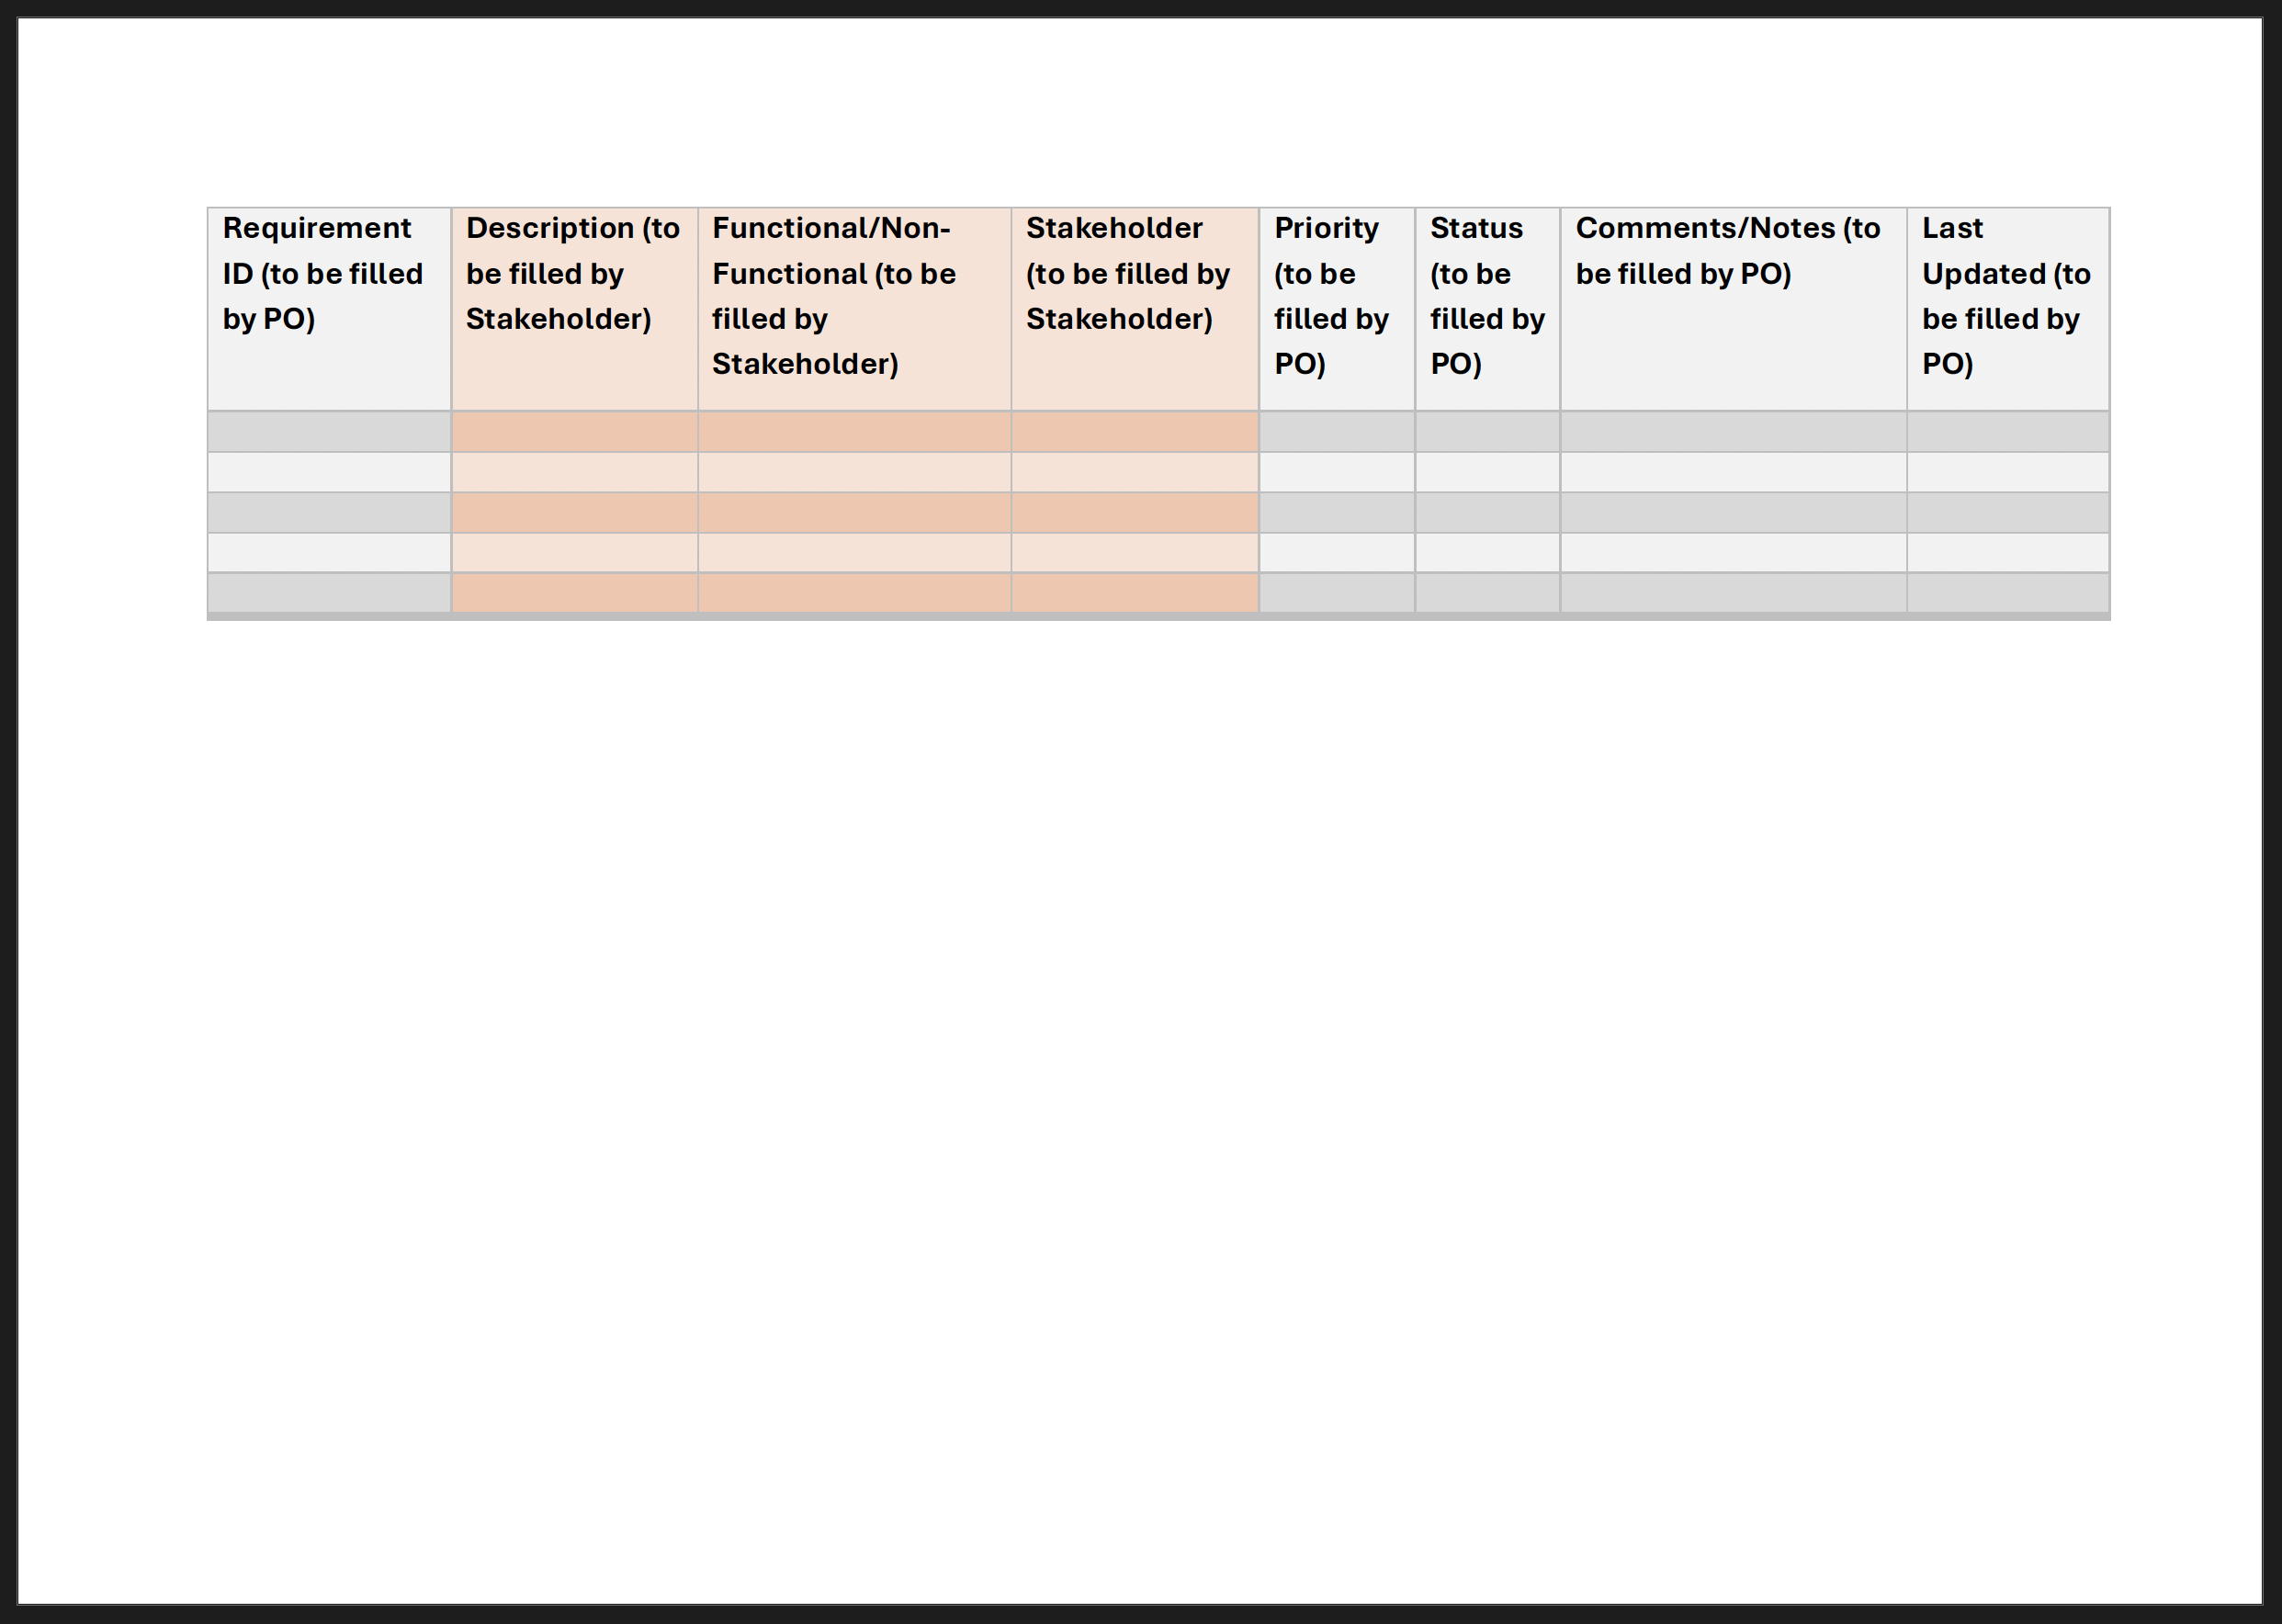
\includegraphics[width=1\textwidth]{abbildungen/RE/Word/RequirementDocument1}
\end{figure}
\begin{figure}[H]
    \centering
    \caption[]{Requirement Document (Page 2)}
    \label{fig:requirement-document-2}
    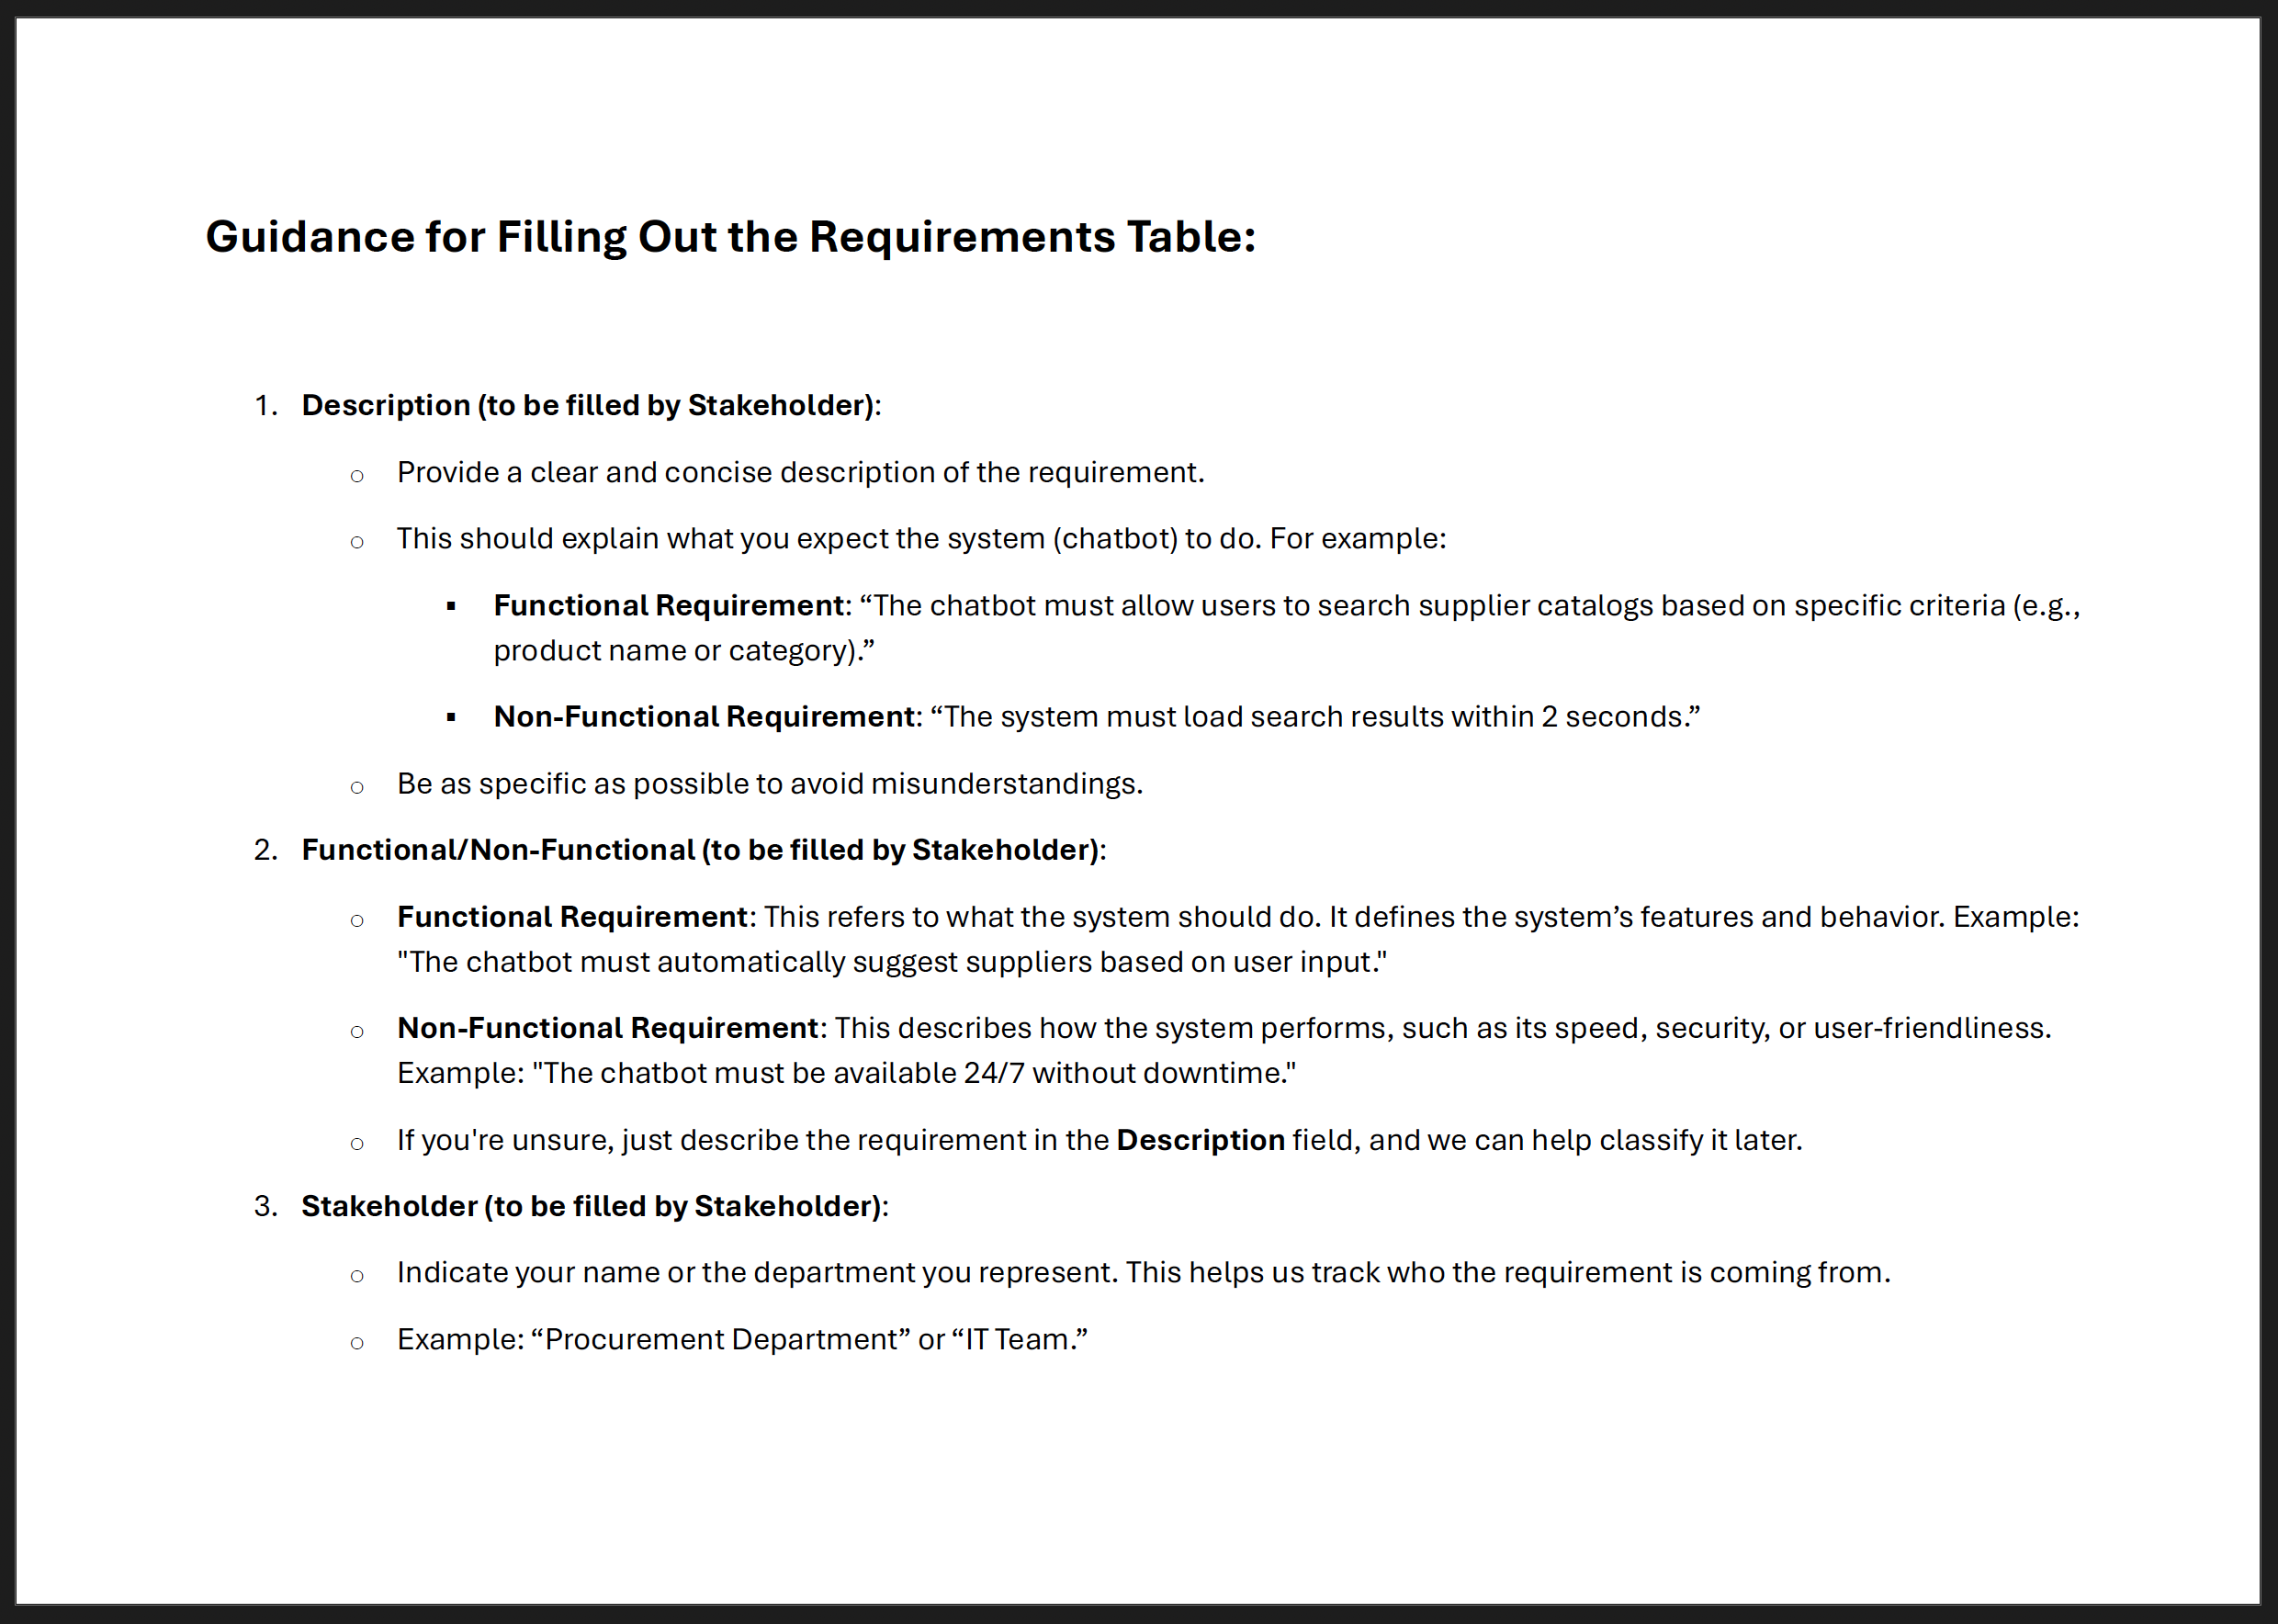
\includegraphics[width=1\textwidth]{abbildungen/RE/Word/RequirementDocument2}
\end{figure}

\section{Requirement Elicitation}\label{sec:requirement-elicitation}
\subsection{Screen Mock-Ups in Miro}\label{subsec:screen-mock-ups-in-miro}
\subsection{Screen Prototypes in Figma}\label{subsec:screen-prototypes-in-figma}
\subsection{Filled-out Requirement Documents}\label{subsec:filled-out-requirement-documents}
\end{appendices}
\addtocontents{toc}{\protect\setcounter{tocdepth}{2}}

%-----------------------------------
% Literaturverzeichnis
%-----------------------------------
\newpage

% Die folgende Zeile trägt ALLE Werke aus literatur.bib in das
% Literaturverzeichnis ein, egal ob sie zietiert wurden oder nicht.
% Der Befehl ist also nur zum Test der Skripte sinnvoll und muss bei echten
% Arbeiten entfernt werden.
%\nocite{*}

%\addcontentsline{toc}{section}{Literatur}

% Die folgenden beiden Befehle würden ab dem Literaturverzeichnis wieder eine
% römische Seitennummerierung nutzen.
% Das ist nach dem Leitfaden nicht zu tun. Dort steht nur dass 'sämtliche
% Verzeichnisse VOR dem Textteil' römisch zu nummerieren sind. (vgl. S. 3)
%\pagenumbering{Roman} %Zähler wieder römisch ausgeben
%\setcounter{page}{4}  %Zähler manuell hochsetzen

% Ausgabe des Literaturverzeichnisses

% Keine Trennung der Werke im Literaturverzeichnis nach ihrer Art
% (Online/nicht-Online)
%\begin{RaggedRight}
%\printbibliography
%\end{RaggedRight}

% Alternative Darstellung, die laut Leitfaden genutzt werden sollte.
% Dazu die Zeilen auskommentieren und folgenden code verwenden:

% Literaturverzeichnis getrennt nach Nicht-Online-Werken und Online-Werken
% (Internetquellen).
% Die Option nottype=online nimmt alles, was kein Online-Werk ist.
% Die Option heading=bibintoc sorgt dafür, dass das Literaturverzeichnis im
% Inhaltsverzeichnis steht.
% Es ist übrigens auch möglich mehrere type- bzw. nottype-Optionen anzugeben, um
% noch weitere Arten von Zusammenfassungen eines Literaturverzeichnisse zu
% erzeugen.
% Beispiel: [type=book,type=article]
\printbibliography[nottype=online,heading=bibintoc,title={\langde{Literaturverzeichnis}\langen{Bibliography}}]

% neue Seite für Internetquellen-Verzeichnis
\newpage

% Laut Leitfaden 2018, S. 14, Fussnote 44 stehen die Internetquellen NICHT im
% Inhaltsverzeichnis, sondern gehören zum Literaturverzeichnis.
% Die Option heading=bibintoc würde die Internetquelle als eigenen Eintrag im
% Inhaltsverzeicnis anzeigen.
%\printbibliography[type=online,heading=bibintoc,title={\headingNameInternetSources}]
\printbibliography[type=online,heading=subbibliography,title={\headingNameInternetSources}]

\newpage
\pagenumbering{gobble} % Keine Seitenzahlen mehr

%-----------------------------------
% Ehrenwörtliche Erklärung
%-----------------------------------
\section*{%
	\langde{Ehrenwörtliche Erklärung}
	\langen{Declaration in lieu of oath}}
\langde{Hiermit versichere ich, dass die vorliegende Arbeit von mir selbstständig und ohne unerlaubte Hilfe angefertigt worden ist, insbesondere dass ich alle Stellen, die wörtlich oder annähernd wörtlich aus Veröffentlichungen entnommen sind, durch Zitate als solche gekennzeichnet habe. Ich versichere auch, dass die von mir eingereichte schriftliche Version mit der digitalen Version übereinstimmt. Weiterhin erkläre ich, dass die Arbeit in gleicher oder ähnlicher Form noch keiner Prüfungsbehörde/Prüfungsstelle vorgelegen hat. Ich erkläre mich damit nicht einverstanden, dass die Arbeit der Öffentlichkeit zugänglich gemacht wird. Ich erkläre mich damit einverstanden, dass die Digitalversion dieser Arbeit zwecks Plagiatsprüfung auf die Server externer Anbieter hochgeladen werden darf. Die Plagiatsprüfung stellt keine Zurverfügungstellung für die Öffentlichkeit dar.}
\langen{I hereby declare that I produced the submitted paper with no assistance from any other party and without the use of any unauthorized aids and, in particular, that I have marked as quotations all passages which are reproduced verbatim or near-verbatim from publications. Also, I declare that the submitted print version of this thesis is identical with its digital version. Further, I declare that this thesis has never been submitted before to any examination board in either its present form or in any other similar version. I herewith disagree that this thesis may be published. I herewith consent that this thesis may be uploaded to the server of external contractors for the purpose of submitting it to the contractors’ plagiarism detection systems. Uploading this thesis for the purpose of submitting it to plagiarism detection systems is not a form of publication.}


\par\medskip
\par\medskip

\vspace{5cm}

\begin{table}[H]
	\centering
	\begin{tabular*}{\textwidth}{c @{\extracolsep{\fill}} ccccc}
		\myOrt, \the\day.\the\month.\the\year
		&
		% Hinterlege deine eingescannte Unterschrift im Verzeichnis /abbildungen und nenne sie unterschrift.png
		% Bilder mit transparentem Hintergrund können teils zu Problemen führen
		\includegraphics[width=0.35\textwidth]{unterschrift}\vspace*{-0.35cm}
		\\
		\rule[0.5ex]{12em}{0.55pt} & \rule[0.5ex]{12em}{0.55pt} \\
		\langde{(Ort, Datum)}\langen{(Location, Date)} & \langde{(Eigenhändige Unterschrift)}\langen{(handwritten signature)}
		\\
	\end{tabular*} \\
\end{table}

\end{document}

%TC:endignore - benötigt für Wordcount in Overleaf